% chktex-file 44
\section*{6. Requisitos}

\subsection{6.1 Alcance detallado}

El sistema a desarrollar es una plataforma web para Fantasy Football orientada al análisis predictivo 
del rendimiento de jugadores y a la recomendación de decisiones de gestión, accesible desde navegador y 
con un modelo de acceso progresivo (funcionalidades públicas y funcionalidades avanzadas para usuarios 
autenticados). En concreto, el alcance incluye:

\begin{itemize}
  \item Visualización de información pública de competición: clasificación, equipos, plantillas y vistas 
  detalladas de equipos y jugadores (estadísticas históricas y rendimiento reciente).
  \item Predicción de puntuación de jugadores para la próxima jornada, incluyendo presentación de un 
  margen de error y explicación de los factores más influyentes (XAI).
  \item Recomendaciones automáticas para apoyar decisiones de mánager: recomendaciones por posición 
  (``Top 3''), asistente de gestión (mantener/vender/fichar) y panel de análisis del próximo rival.
  \item Funcionalidades para usuarios registrados: creación de cuenta, autenticación, gestión de perfil y 
  persistencia de una plantilla personalizada con formación, proyección de puntuación y alertas básicas.
  \item Acceso a histórico y simulación/retro-evaluación (backtesting funcional) para comparar predicción 
  vs resultado en jornadas pasadas.
\end{itemize}

\subsection{6.2 Fuera de alcance}

Para acotar la complejidad, se consideran fuera de alcance en esta versión del proyecto:

\begin{itemize}
  \item Integración oficial con LaLiga Fantasy (login, mercado real, transacciones reales o sincronización 
  automática) ya que no existe API pública estable.
  \item Predicción de evolución del valor de mercado (ya identificado como limitación por ausencia de 
  histórico consistente).
  \item Modelado explícito de lesiones/rotaciones/rumores en tiempo real (se tratará como limitación del 
  modelo y del dominio).
  \item Notificaciones push móviles y apps móvil dedicada.
\end{itemize}

\subsection{6.3 Suposiciones, dependencias y restricciones}

\begin{itemize}
  \item Dependencia de disponibilidad y estabilidad de fuentes externas (APIs/HTML/CSV); cambios de 
  formato pueden requerir adaptación del pipeline.
  \item Restricción de idioma: interfaz y mensajes en castellano (RNF1).
  \item Restricción de rendimiento: objetivo de tiempos de respuesta (RNF3) sujeto a condiciones de 
  prueba controladas.
  \item Se considerará que todos los jugadores están disponibles y en forma durante toda la temporada.
\end{itemize}

\subsection{6.4 Actores}

En el modelo de casos de uso de la plataforma se consideran únicamente actores humanos, diferenciando 
entre actores primarios (persiguen un objetivo directo con el sistema) y actores de soporte (interactúan 
para administración/supervisión).

\subsubsection{6.4.1 Usuario anónimo}

\textbf{Objetivo:} Consultar información pública y explorar jugadores y equipos sin crear una cuenta.

\textbf{Interacciones típicas:}
\begin{itemize}
  \item Ver clasificación y páginas públicas de equipos/jugadores (RF1, RF2, RF3).
  \item Buscar por nombre y aplicar filtros básicos (RF4).
  \item Consultar fichas y paneles informativos accesibles sin autenticación (RF5).
\end{itemize}

\subsubsection{6.4.2 Usuario registrado (Mánager)}

\textbf{Objetivo:} Gestionar su plantilla y tomar decisiones apoyadas por predicciones, recomendaciones 
y explicaciones.

\textbf{Interacciones típicas:}
\begin{itemize}
  \item Registrarse, iniciar/cerrar sesión y gestionar su cuenta (RF6).
  \item Crear/editar su plantilla y formación; ver proyección agregada (RF7, RF8).
  \item Consultar predicciones con explicación (XAI) (RF8, RF9).
  \item Consultar recomendaciones por posición y asistente de gestión (RF10, RF11).
  \item Acceder a histórico y simulación en jornadas pasadas (RF12).
  \item Configurar visibilidad de plantilla y usar funcionalidades sociales (RF13, RF14).
  \item Recibir notificaciones/alertas (RF15).
\end{itemize}

\subsection{6.5 Requisitos funcionales}

Para la priorización de los requisitos del sistema se utilizará el método \textit{MoSCoW}, una técnica ampliamente 
empleada en la gestión de proyectos que permite clasificar los requisitos en función de su importancia y 
necesidad. 

\newcommand{\RFTable}[5]{%
\begin{table}[H]
  \centering
  \renewcommand{\arraystretch}{1.18}
  \begin{tabular}{@{}|>{\centering\arraybackslash}p{0.09\linewidth}|>{\raggedright\arraybackslash}p{0.43\linewidth}|>{\raggedright\arraybackslash}p{0.43\linewidth}|@{}}
    \hline
    \textbf{ID} & \textbf{Descripción} & \textbf{Historia de usuario} \\
    \hline
    \multirow{3}{*}{\textbf{#1}} & \rule{0pt}{4.2ex}#2 & \begingroup\let\\\newline #3\endgroup \\
    \cline{2-3}
    & \textbf{Información del Requisito} & \textbf{Criterios de aceptación} \\
    \cline{2-3}
    & \rule{0pt}{4.2ex}\begingroup\let\\\newline #4\endgroup & \begingroup\let\\\newline #5\endgroup \\
    \hline
  \end{tabular}
  \renewcommand{\arraystretch}{1}
\end{table}
}

\RFTable{RF1}
{Visualización de clasificación}
{\textbf{Como:} Usuario anónimo\\ \textbf{Quiero:} Ver la clasificación de la liga y su evolución por jornada\\ \textbf{Para:} Entender el estado actual de la competición sin salir de la aplicación}
{\textbf{Actor:} Usuario anónimo\\ \textbf{Auth:} No\\ \textbf{Prioridad:} Must Have}
{CA1.1. La clasificación muestra posición, nombre, puntos, racha reciente, goles a favor, en contra y diferencia de goles.\\ CA1.2. Al menos el 95\% de los datos están disponibles y correctos.}

\RFTable{RF2}
{Ficha de equipo}
{\textbf{Como:} Usuario anónimo\\ \textbf{Quiero:} Ver la plantilla y detalles de un equipo\\ \textbf{Para:} Conocer su estado actual}
{\textbf{Actor:} Usuario anónimo\\ \textbf{Auth:} No\\ \textbf{Prioridad:} Must Have}
{CA2.1. Acceso desde clasificación o buscador.\\ CA2.2. Muestra plantilla con enlaces a fichas de jugadores.\\ CA2.3. Muestra próximo rival y panel de análisis.}

\RFTable{RF3}
{Ficha de jugador}
{\textbf{Como:} Usuario anónimo\\ \textbf{Quiero:} Ver información detallada de un jugador\\ \textbf{Para:} Analizar su rendimiento}
{\textbf{Actor:} Usuario anónimo\\ \textbf{Auth:} No\\ \textbf{Prioridad:} Must Have}
{CA3.1. Muestra estadísticas históricas del jugador.\\ CA3.2. Incluye datos de temporadas anteriores.\\ CA3.3. Incluye puntos acumulados de la temporada actual.}

\RFTable{RF4}
{Buscador de equipos y jugadores}
{\textbf{Como:} Usuario anónimo\\ \textbf{Quiero:} Buscar jugadores o equipos rápidamente\\ \textbf{Para:} Encontrarlos sin navegar manualmente}
{\textbf{Actor:} Usuario anónimo\\ \textbf{Auth:} No\\ \textbf{Prioridad:} Must Have}
{CA4.1. Permite búsqueda por texto parcial.\\ CA4.2. Ofrece autocompletado a partir de 3 caracteres.}

\RFTable{RF5}
{Panel próximo rival}
{\textbf{Como:} Usuario anónimo\\ \textbf{Quiero:} Ver el análisis del próximo rival\\ \textbf{Para:} Entender el contexto táctico del partido}
{\textbf{Actor:} Usuario anónimo\\ \textbf{Auth:} No\\ \textbf{Prioridad:} Should Have}
{CA5.1. Incluye métricas de últimas 5 jornadas (GF, GC, racha).\\ CA5.2. Incluye histórico de enfrentamientos previos (H2H).}

\RFTable{RF6}
{Registro e inicio/cierre sesión}
{\textbf{Como:} Usuario anónimo\\ \textbf{Quiero:} Crear una cuenta e iniciar sesión\\ \textbf{Para:} Acceder a funcionalidades personalizadas}
{\textbf{Actor:} Usuario anónimo\\ \textbf{Auth:} No\\ \textbf{Prioridad:} Must Have}
{CA6.1. Valida correctamente los campos.\\ CA6.2. Muestra mensajes de error informativos.\\ CA6.3. Permite eliminar cuenta de usuario.}

\RFTable{RF7}
{Gestión de fantasy}
{\textbf{Como:} Usuario registrado\\ \textbf{Quiero:} Gestionar mi plantilla de Fantasy\\ \textbf{Para:} Hacer seguimiento estratégico de mis jugadores}
{\textbf{Actor:} Usuario registrado\\ \textbf{Auth:} Sí\\ \textbf{Prioridad:} Must Have}
{CA7.1. Permite añadir y eliminar jugadores de plantilla.\\ CA7.2. Mantiene persistencia de cambios.\\ CA7.3. Ofrece interfaz familiar y accesible.\\ CA7.4. Soporta múltiples formaciones.}

\RFTable{RF8}
{Gestión de plantillas}
{\textbf{Como:} Usuario registrado\\ \textbf{Quiero:} Gestionar múltiples plantillas\\ \textbf{Para:} Organizar escenarios y estrategias}
{\textbf{Actor:} Usuario registrado\\ \textbf{Auth:} Sí\\ \textbf{Prioridad:} Must Have}
{CA8.1. Permite crear nuevas plantillas.\\ CA8.2. Permite renombrar plantillas existentes.\\ CA8.3. Permite definir plantilla predeterminada.}

\RFTable{RF9}
{Predicción de puntos de cada jugador}
{\textbf{Como:} Usuario registrado\\ \textbf{Quiero:} Ver los puntos predichos de mi plantilla\\ \textbf{Para:} Decidir mi alineación óptima}
{\textbf{Actor:} Usuario registrado\\ \textbf{Auth:} Sí\\ \textbf{Prioridad:} Must Have}
{CA9.1. Muestra puntos predichos en Mi Plantilla.\\ CA9.2. Permite seleccionar jornada desde la interfaz.\\ CA9.3. Informa motivo si no hay predicción.\\ CA9.4. Muestra proyección total de plantilla.}

\RFTable{RF10}
{Explicabilidad de las predicciones}
{\textbf{Como:} Usuario registrado\\ \textbf{Quiero:} Entender la predicción de mis jugadores\\ \textbf{Para:} Aumentar mi confianza en el sistema}
{\textbf{Actor:} Usuario registrado\\ \textbf{Auth:} Sí\\ \textbf{Prioridad:} Must Have}
{CA10.1. Muestra top 3 \textit{features} más influyentes.\\ CA10.2. Describe contribución de cada \textit{feature}.\\ CA10.3. Muestra aviso si la explicación no está disponible.}

\RFTable{RF11}
{Recomendaciones por posición (Top 3)}
{\textbf{Como:} Usuario registrado\\ \textbf{Quiero:} Ver candidatos destacados por posición\\ \textbf{Para:} Tomar mejores decisiones de fichaje}
{\textbf{Actor:} Usuario registrado\\ \textbf{Auth:} Sí\\ \textbf{Prioridad:} Should Have}
{CA11.1. Muestra top 3 jugadores por posición.\\ CA11.2. Incluye explicación de la recomendación.\\ CA11.3. Incluye acceso directo a ficha del jugador.}

\RFTable{RF12}
{Asistente de gestión}
{\textbf{Como:} Usuario registrado\\ \textbf{Quiero:} Recibir consejo sobre decisiones de plantilla\\ \textbf{Para:} Optimizar rendimiento en la liga}
{\textbf{Actor:} Usuario registrado\\ \textbf{Auth:} Sí\\ \textbf{Prioridad:} Could Have}
{CA12.1. Permite seleccionar jugador para análisis.\\ CA12.2. Recomienda acción (mantener/vender/fichar).\\ CA12.3. Incluye comparativa y explicación completa.}

\RFTable{RF13}
{Histórico de predicciones}
{\textbf{Como:} Usuario registrado\\ \textbf{Quiero:} Revisar predicciones pasadas\\ \textbf{Para:} Medir la fiabilidad del sistema}
{\textbf{Actor:} Usuario registrado\\ \textbf{Auth:} Sí\\ \textbf{Prioridad:} Could Have}
{CA13.1. Incluye tabla predicho vs real.\\ CA13.2. Muestra métrica agregada de precisión.\\ CA13.3. Explicita control anti \textit{data leakage}.}

\RFTable{RF14}
{Sistema de amistad}
{\textbf{Como:} Usuario registrado\\ \textbf{Quiero:} Enviar, recibir y rechazar solicitudes de amistad\\ \textbf{Para:} Conectar y comparar equipos}
{\textbf{Actor:} Usuario registrado\\ \textbf{Auth:} Sí\\ \textbf{Prioridad:} Could Have}
{CA14.1. Permite envío por nombre o apodo.\\ CA14.2. Permite aceptar o rechazar solicitudes.\\ CA14.3. Evita solicitudes duplicadas activas.}

\RFTable{RF15}
{Visibilidad de plantilla}
{\textbf{Como:} Usuario registrado\\ \textbf{Quiero:} Configurar la visibilidad de mi plantilla\\ \textbf{Para:} Proteger mi estrategia}
{\textbf{Actor:} Usuario registrado\\ \textbf{Auth:} Sí\\ \textbf{Prioridad:} Could Have}
{CA15.1. Permite marcar plantilla como pública o privada.\\ CA15.2. Privada: solo propietario accede.\\ CA15.3. Pública: solo amigos acceden.}

\RFTable{RF16}
{Sistema de notificaciones}
{\textbf{Como:} Usuario registrado\\ \textbf{Quiero:} Recibir notificaciones de eventos relevantes\\ \textbf{Para:} Estar siempre al día}
{\textbf{Actor:} Usuario registrado\\ \textbf{Auth:} Sí\\ \textbf{Prioridad:} Could Have}
{CA16.1. Muestra notificaciones en bandeja.\\ CA16.2. Permite marcar notificaciones como leídas.}

\RFTable{RF17}
{Partidos de la jornada}
{\textbf{Como:} Usuario anónimo\\ \textbf{Quiero:} Ver los partidos de cada jornada\\ \textbf{Para:} Consultar fácilmente el calendario}
{\textbf{Actor:} Usuario anónimo\\ \textbf{Auth:} No\\ \textbf{Prioridad:} Should Have}
{CA17.1. Muestra partidos de la jornada seleccionada.\\ CA17.2. Muestra escudos, horarios y días.\\ CA17.3. Muestra sucesos del partido si ya se jugó.}

\RFTable{RF18}
{Personalización de perfil}
{\textbf{Como:} Usuario registrado\\ \textbf{Quiero:} Personalizar mi perfil\\ \textbf{Para:} Reflejar mi identidad y preferencias}
{\textbf{Actor:} Usuario registrado\\ \textbf{Auth:} Sí\\ \textbf{Prioridad:} Could Have}
{CA18.1. Permite foto de perfil personalizada.\\ CA18.2. Permite seleccionar equipos favoritos.\\ CA18.3. Permite estado personalizado visible.}

\RFTable{RF19}
{Comparativa de jugadores}
{\textbf{Como:} Usuario registrado\\ \textbf{Quiero:} Comparar jugadores en diferentes temporadas\\ \textbf{Para:} Tomar mejores decisiones de fichaje}
{\textbf{Actor:} Usuario registrado\\ \textbf{Auth:} Sí\\ \textbf{Prioridad:} Could Have}
{CA19.1. Permite seleccionar múltiples jugadores.\\ CA19.2. Permite elegir temporadas a comparar.\\ CA19.3. Muestra estadísticas normalizadas por 90 minutos.}

\subsection{6.6 Requisitos no funcionales}

\paragraph{RNF1. Rendimiento y tiempos de respuesta}
~\\
RNF1.1: Consultas estándar en $<$ 500 ms. \\
RNF1.2: Predicción/XAI en $<$ 2 s con modelo precargado.

\paragraph{RNF2. Usabilidad e idioma}
~\\
RNF2.1: Interfaz íntegramente en castellano, incluyendo errores.

\paragraph{RNF3. Calidad del dato y anti data leakage}
~\\
RNF3.1: Features calculadas solo con información anterior al evento predicho.

\paragraph{RNF4. Soporte y explicabilidad para el usuario}
~\\
RNF4.1: Glosario accesible de features/estadísticas. \\
RNF4.2: Nombres legibles en explicaciones con indicación positiva/negativa. \\
RNF4.3: Acceso visible a ayuda e tooltips en pantallas clave.

\paragraph{RNF5. Seguridad y privacidad}
~\\
RNF5.1: Contraseñas con hash seguro + salt (mecanismo del framework). \\
RNF5.2: Sesión cerrada sin acceso a recursos privados sin reautenticación. \\
RNF5.3: Minimización de datos personales (solo username como identificador público).

\subsection{6.7 Casos de uso}

Los casos de uso se modelan considerando dos perfiles: usuario anónimo y usuario registrado. Se presentan mediante diagramas que ilustran las interacciones entre actores y sistema.

\begin{figure}[H]
\centering
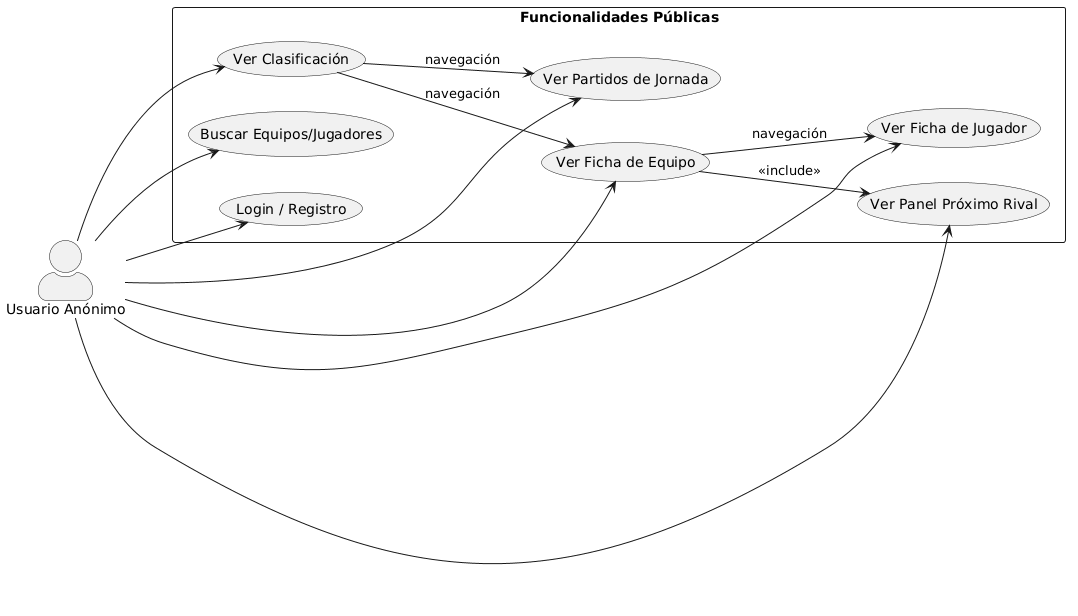
\includegraphics[width=1\textwidth]{images/cu-anonimo.png}
\caption{CU Anónimo.}\label{fig:cu-anonimo}
\end{figure}

\begin{figure}[H]
\centering
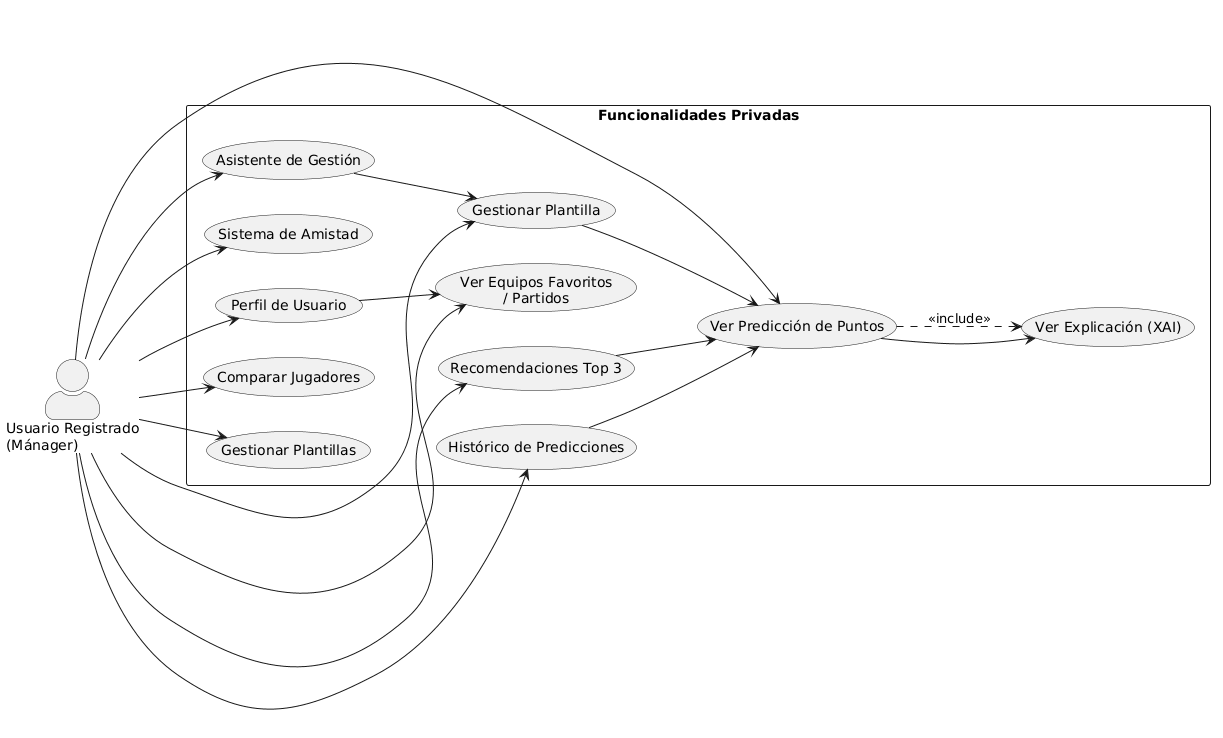
\includegraphics[width=1\textwidth]{images/cu-registrado.png}
\caption{CU Registrado.}\label{fig:cu-registrado}
\end{figure}

\newcommand{\CUTable}[7]{%
\begin{table}[H]
  \centering
  \renewcommand{\arraystretch}{1.18}
  \begin{tabular}{@{}|p{0.49\linewidth}|p{0.49\linewidth}|@{}}
    \hline
    \multicolumn{2}{|p{0.98\linewidth}|}{\textbf{ID:} #1} \\
    \hline
    \textbf{Actores:} #2 & \textbf{Precondiciones:} #3 \\
    \hline
    \textbf{RF Asociados:} #4 & \textbf{Postcondiciones:} #5 \\
    \hline
    \begin{minipage}[t]{\linewidth}\textbf{Flujo principal}\par\vspace{2pt}#6\vspace{0.5em}\end{minipage} & \begin{minipage}[t]{\linewidth}\textbf{Flujo alternativo/excepciones}\par\vspace{2pt}#7\vspace{0.5em}\end{minipage} \\
    \hline
  \end{tabular}
  \renewcommand{\arraystretch}{1}
\end{table}
}

\newcommand{\CUOneMain}{El usuario accede a ``Liga'' $\to$ Sistema carga jornada actual $\to$ Se muestran equipos, posición, puntos, racha, GF, GC $\to$ (Opcional) Usuario cambia jornada $\to$ Se refresca tabla.}
\newcommand{\CUOneAlt}{Si jornada futura: se cargan partidos y estado de última jornada completa.}
\newcommand{\CUTwoMain}{Selecciona equipo $\to$ Se abre ficha $\to$ Se muestra plantilla (jugadores + posiciones) $\to$ Se muestra próximo rival $\to$ Usuario abre análisis $\to$ Se muestran métricas y H2H.}
\newcommand{\CUTwoAlt}{Sin próximo rival: ``No disponible''. Sin H2H: ``Histórico no disponible'' sin error.}
\newcommand{\CUThreeMain}{Usuario entra a ficha $\to$ Se muestran estadísticas y últimas 8 jornadas $\to$ Consulta temporadas anteriores $\to$ Se cargan datos adicionales.}
\newcommand{\CUThreeAlt}{Sin temporadas anteriores: sección oculta. Jugador no encontrado: error 404 funcional.}
\newcommand{\CUFourMain}{Accede a ``Mi plantilla'' $\to$ Se carga plantilla guardada $\to$ Añade/elimina jugadores y elige formación $\to$ Sistema guarda cambios $\to$ Se muestran puntos predichos + incertidumbre $\to$ Usuario abre detalle de jugador $\to$ Se muestran top 3 features.}
\newcommand{\CUFourAlt}{Sin predicción: muestra motivo. Sin explicación: ``No disponible'' manteniendo predicción. Datos insuficientes: media previa.}

\CUTable%
{CU1 - Consultar clasificación de LaLiga}
{Usuario anónimo}
{Ninguna}
{RF1}
{Se muestra la clasificación.}
{1. El usuario accede a “Liga”.\\2. El sistema carga la jornada por defecto (actual).\\3. El sistema muestra equipos, posición, puntos, racha, GF, GC…\\4. (Opcional) El usuario cambia la jornada.\\5. El sistema refresca la tabla.}
{A1. El usuario navega a una jornada en el futuro, en dicho caso, se cargan los partidos de la jornada y el estado de la última jornada completa.}

\CUTable%
{CU2 - Consultar ficha de equipo}
{Usuario anónimo}
{Ninguna}
{RF2, RF5}
{Se muestra la ficha del equipo y el panel de su próximo rival.}
{1. El usuario selecciona un equipo desde clasificación o buscador.\\2. El sistema abre la ficha del equipo.\\3. El sistema muestra plantilla (jugadores + posiciones) y enlaces a fichas individuales.\\4. El sistema muestra próximo rival.\\5. El usuario abre el análisis del rival.\\6. El sistema muestra métricas del rival y H2H.}
{A1. No hay datos de próximo rival: se muestra “Próximo rival no disponible”.\\A2. No hay datos H2H: se muestra “Histórico no disponible” sin error.}

\CUTable%
{CU3 - Consultar ficha de jugador}
{Usuario anónimo}
{Ninguna}
{RF3}
{Se muestra ficha del jugador o estado “No disponible”.}
{1. El usuario entra a la ficha del jugador (desde equipo o buscador).\\2. El sistema muestra estadísticas históricas y últimas 8 jornadas.\\3. El usuario consulta temporadas anteriores (si existen).\\4. El sistema muestra los datos adicionales.}
{A1. Sin datos de temporadas anteriores: se oculta sección o muestra “Sin registros”.\\A2. Jugador no encontrado: se muestra 404 funcional (“Jugador no encontrado”).}

\CUTable%
{CU4 - Gestionar plantilla y ver predicción con XAI}
{Usuario registrado}
{Usuario autenticado.}
{RF7, RF8, RF9}
{Plantilla guardada y XAI y predicciones mostradas.}
{1. El usuario accede a “Mi plantilla”.\\2. El sistema carga la plantilla guardada.\\3. El usuario añade/elimina jugadores y elige formación.\\4. El sistema guarda cambios.\\5. El sistema muestra puntos predichos + incertidumbre y proyección total.\\6. El usuario abre el detalle de un jugador.\\7. El sistema muestra top 3 features por su contribución.}
{A1. Sin predicción para un jugador: se muestra motivo en ese jugador.\\A2. Explicación no disponible: se muestra aviso “Explicación no disponible” manteniendo la predicción.\\A3. Si no existen suficientes datos previos simplemente se mostrará la media previa al partido.}

\begin{figure}[H]
\centering
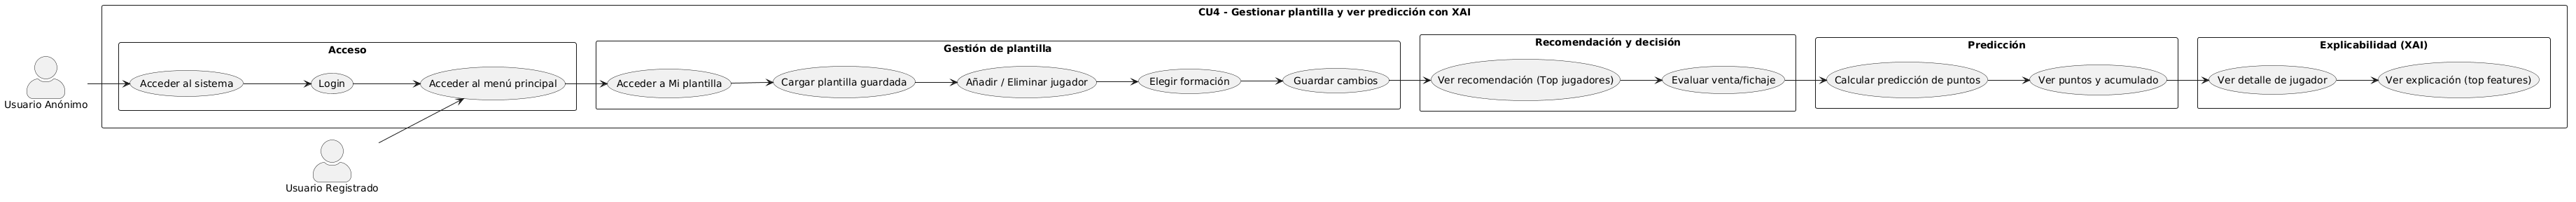
\includegraphics[width=1\textwidth]{images/cu4.png}
\caption{Flujo de usuario en el caso de uso 4.}\label{fig:cu4}
\end{figure}


\subsection{6.8 Prototipado de UI}


Para la elaboración de los mockups y la versión inicial de las vistas de la aplicación se utilizó la herramienta de inteligencia artificial Stitch (https://stitch.withgoogle.com/). 
Esta herramienta permite generar interfaces a partir de descripciones textuales detalladas, lo que facilitó la creación de diseños alineados 
con los requisitos funcionales y la idea conceptual del proyecto.\par

Se optó por esta solución debido a que, además de generar una imagen en formato PNG, también proporciona automáticamente el código HTML junto con su CSS asociado, 
lo que supone una ventaja significativa en términos de productividad.\par

Esta funcionalidad permite avanzar directamente hacia una implementación real de la interfaz, reduciendo considerablemente el esfuerzo necesario en comparación con
 otras alternativas, como el uso de herramientas de diseño estático (por ejemplo, Canva) o el desarrollo manual desde cero del HTML y CSS.
Gracias a este enfoque, se ha conseguido acelerar la fase de prototipado y reducir el tiempo de desarrollo, manteniendo al mismo tiempo una coherencia entre el 
diseño inicial y la implementación final de la interfaz.

\begin{figure}[H]
\centering
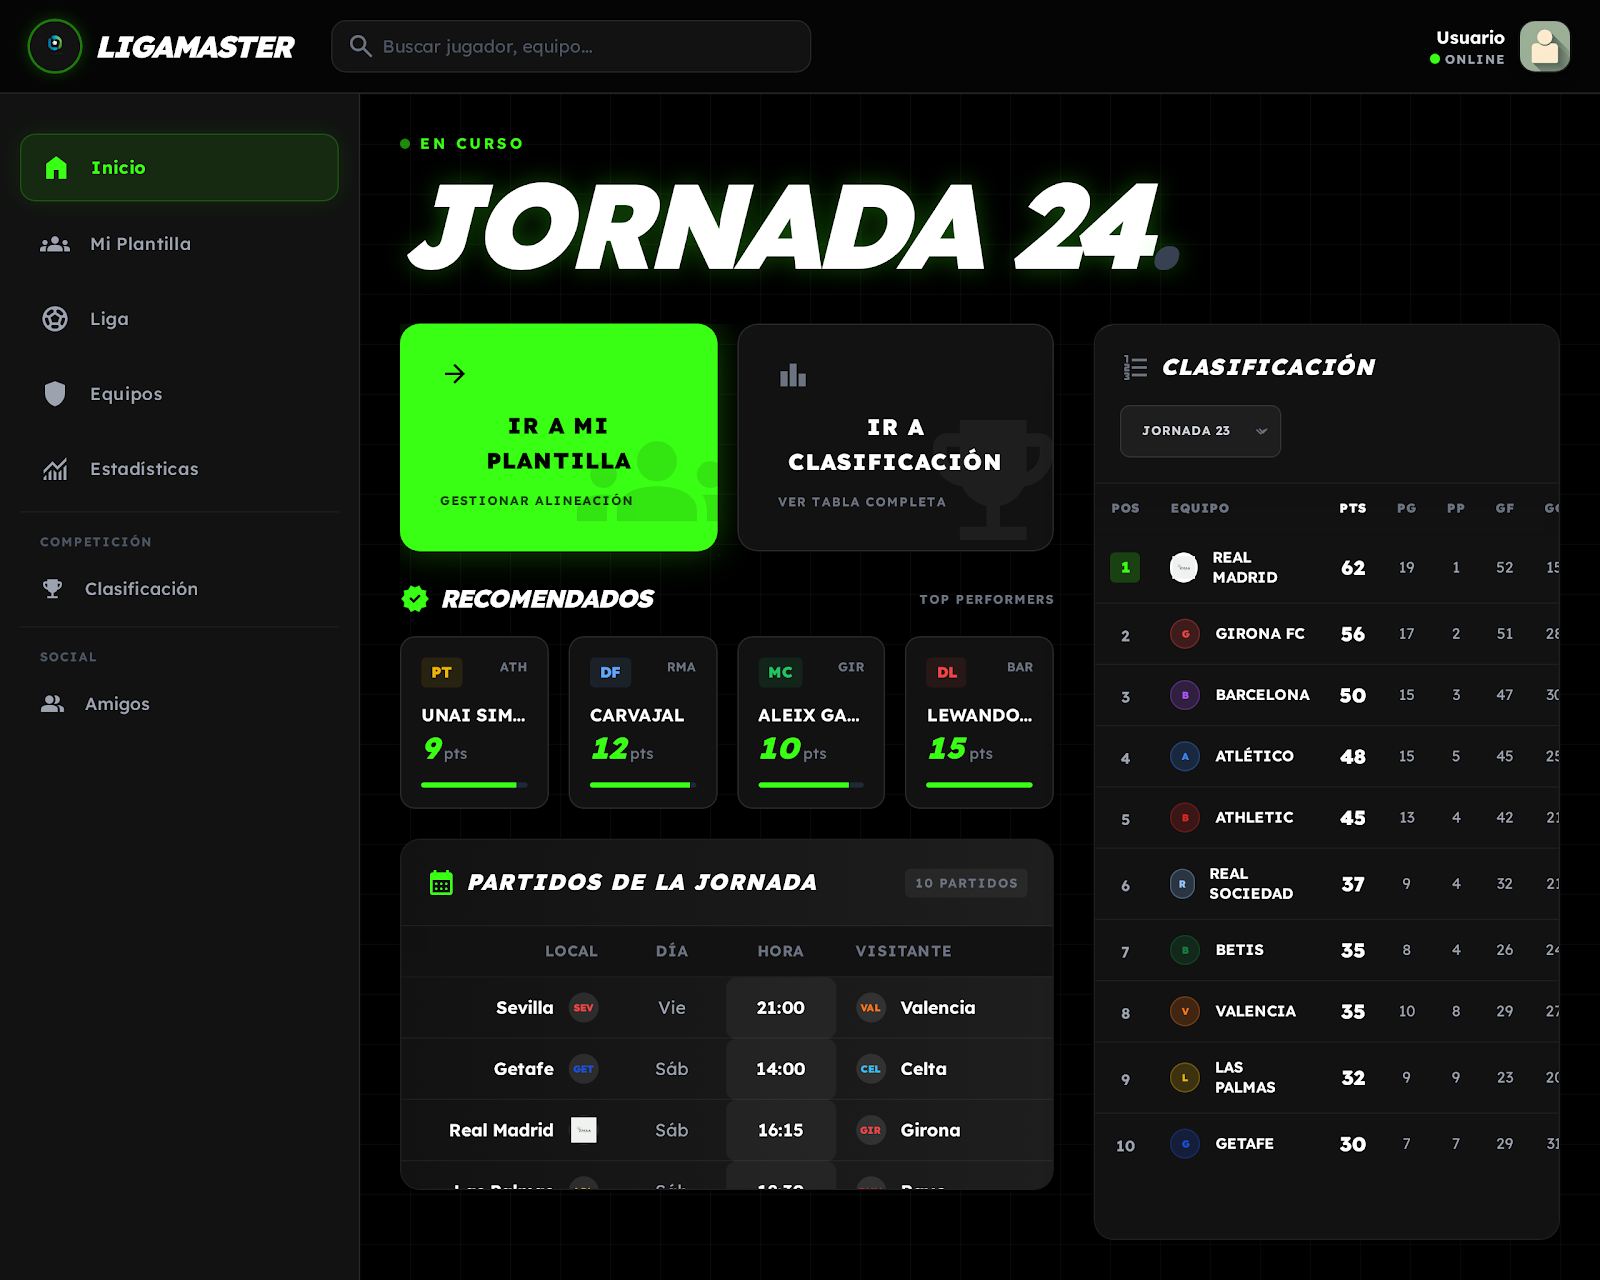
\includegraphics[width=0.6\textwidth]{images/mockups/menu.png}
\caption{Prototipo del menú principal de la aplicación, con algunas funcionalidades y donde el usuario puede navegar entre las distintas secciones desde la barra lateral.}
\label{fig:mockup-menu}
\end{figure}

\begin{figure}[H]
\centering
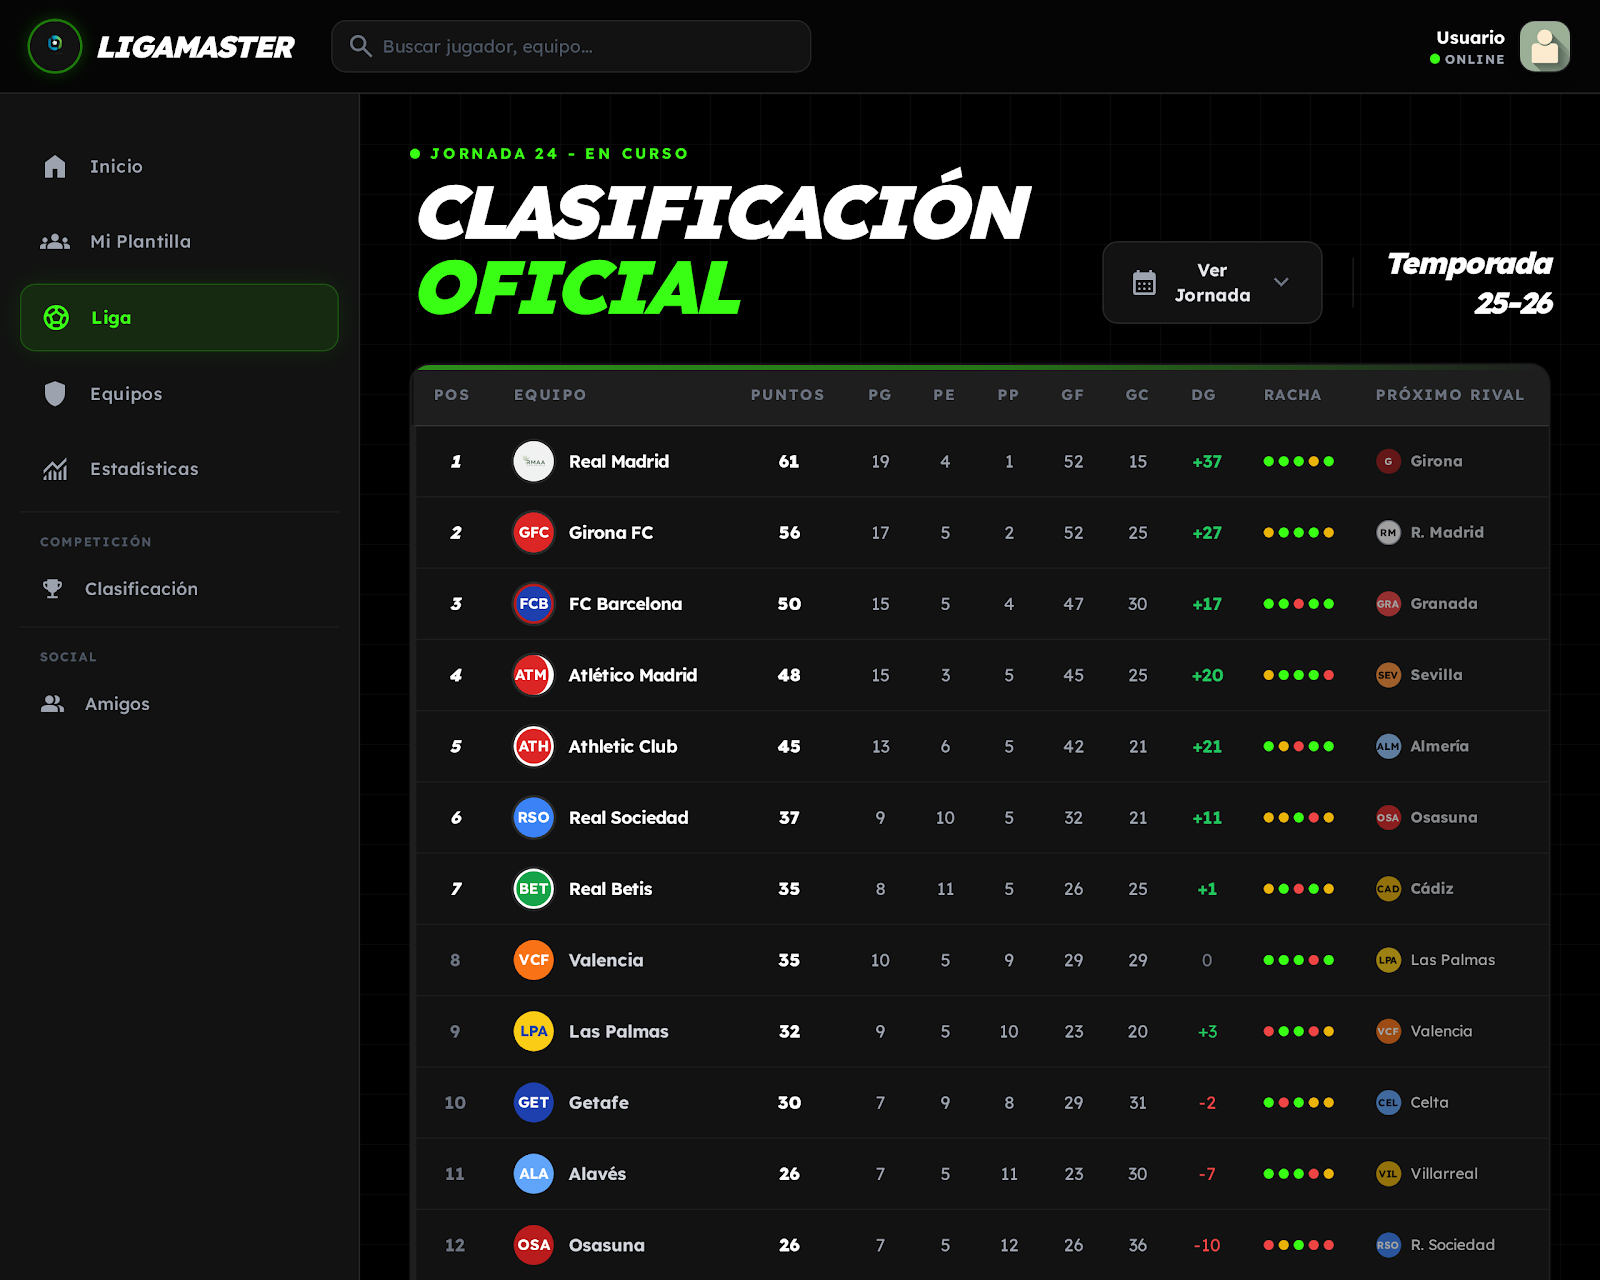
\includegraphics[width=0.6\textwidth]{images/mockups/clasificacion.png}
\caption{Prototipo de clasificación de LaLiga, mostrando equipos, posiciones y puntos.}
\label{fig:mockup-clasificacion}
\end{figure}

\begin{figure}[H]
\centering
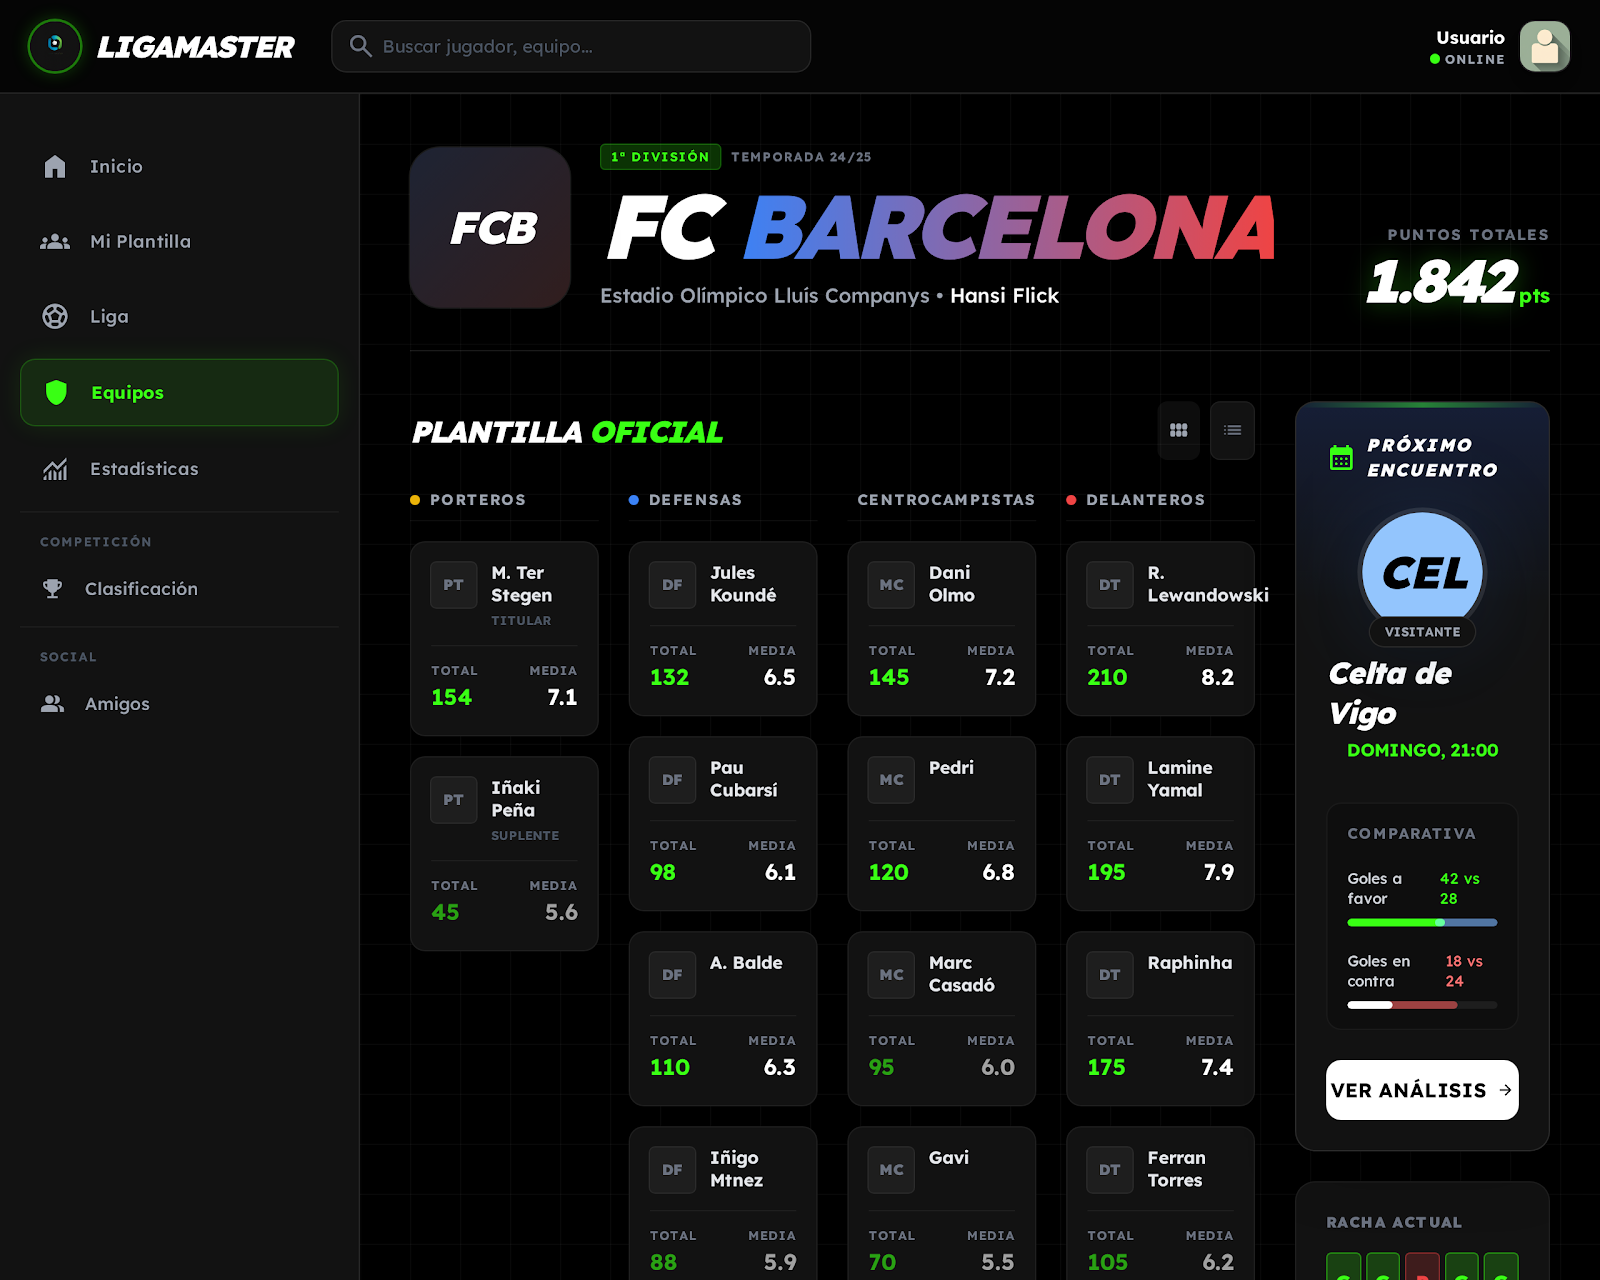
\includegraphics[width=0.6\textwidth]{images/mockups/equipo.png}
\caption{Prototipo de la ficha de equipo, con plantilla, posiciones, próximo partido y acceso a detalles individuales de los jugadores.}
\label{fig:mockup-equipo}
\end{figure}

\begin{figure}[H]
\centering
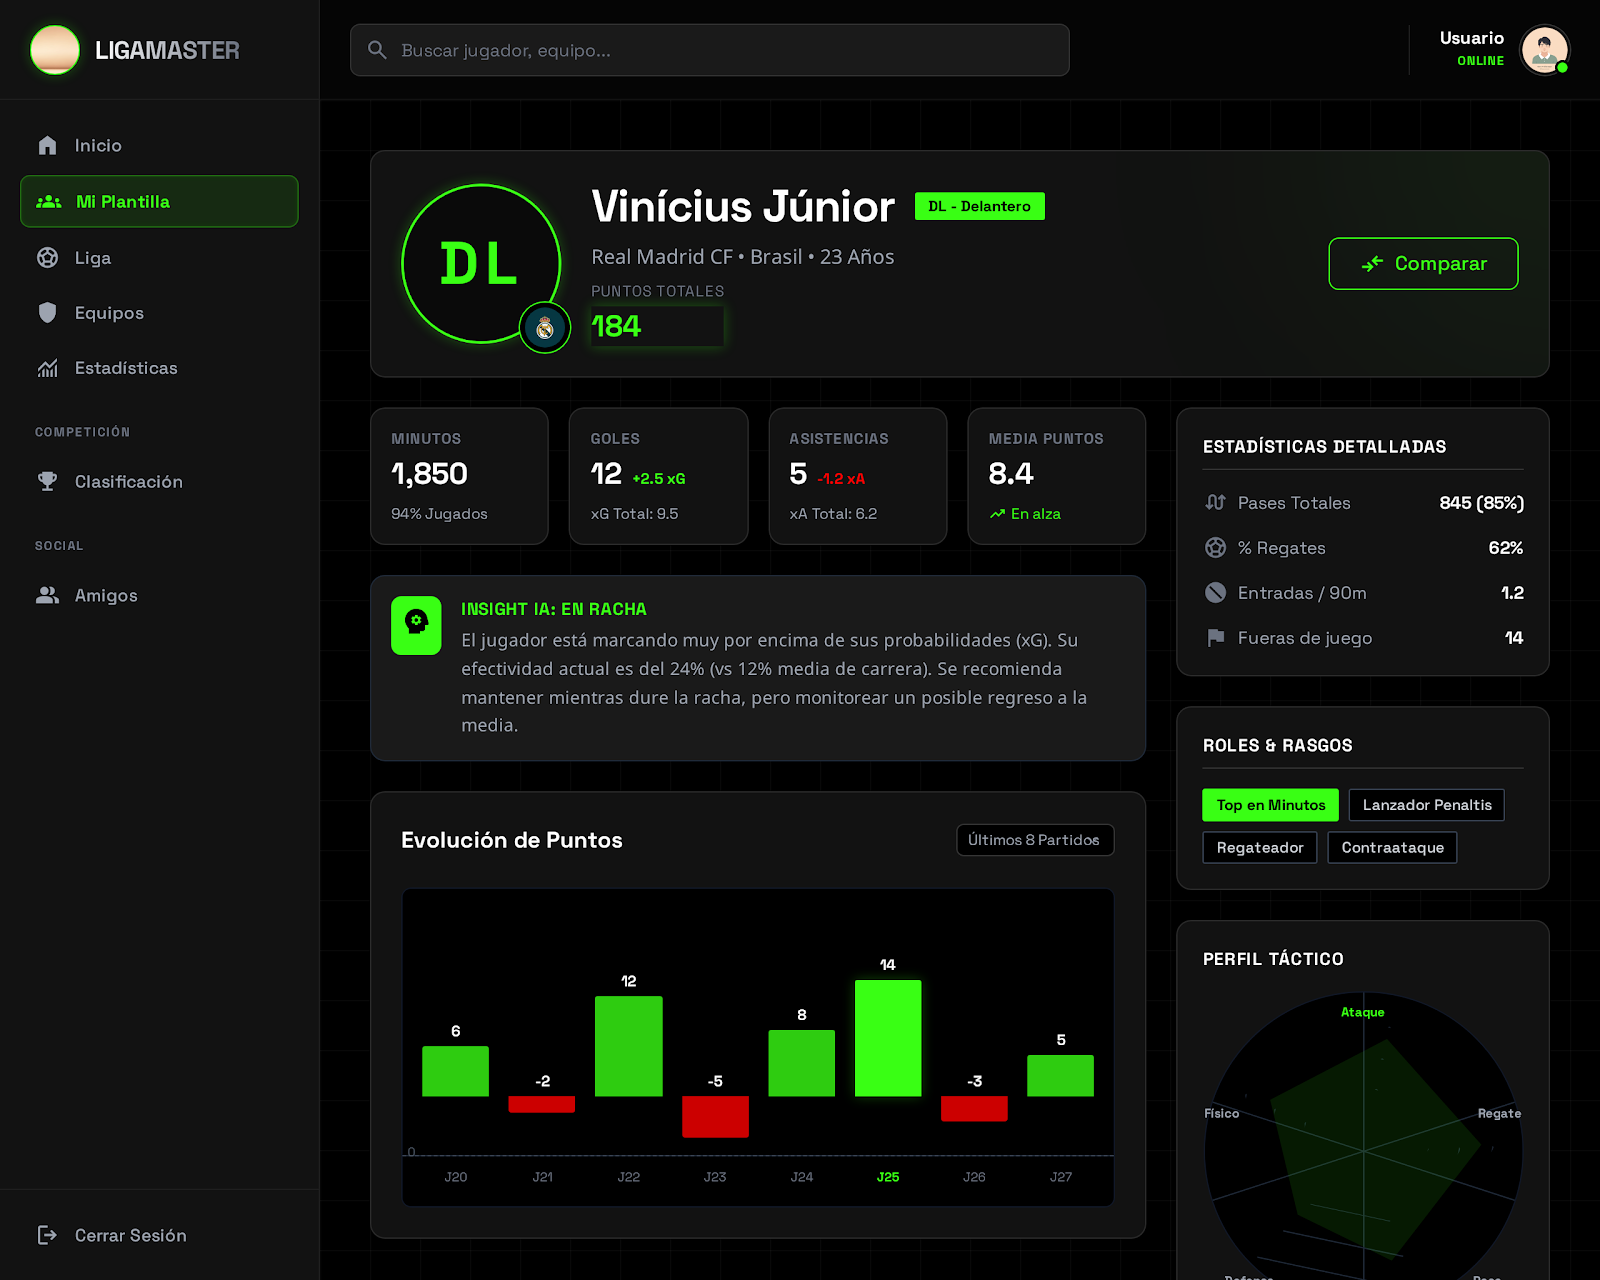
\includegraphics[width=0.6\textwidth]{images/mockups/jugador.png}
\caption{Protipo de la vista de jugador, mostrando estadísticas históricas y rendimiento reciente.}
\label{fig:mockup-jugador}
\end{figure}

\begin{figure}[H]
\centering
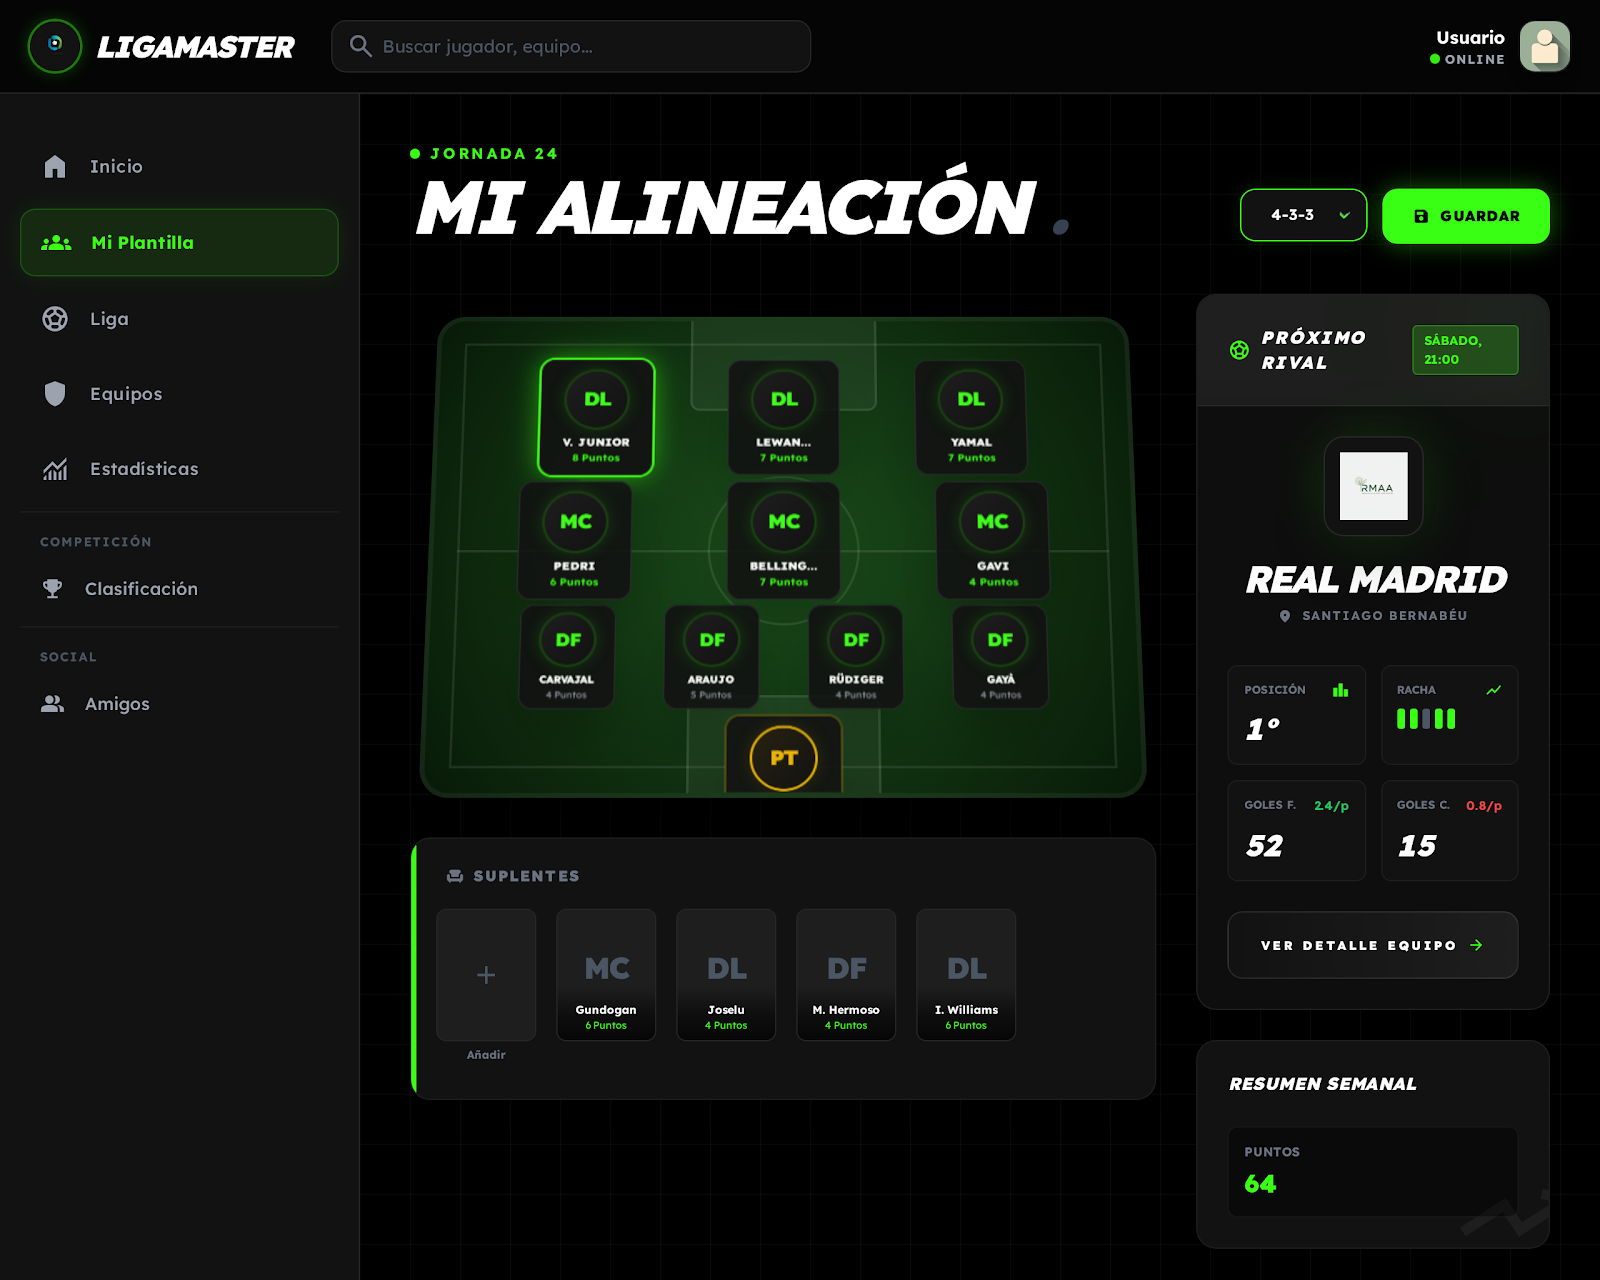
\includegraphics[width=0.6\textwidth]{images/mockups/plantilla.png}
\caption{Prototipo de la vista de plantilla de usuario, con predicción de puntos y explicación XAI.}
\label{fig:mockup-plantilla}
\end{figure}


